\chapter{Methods}\label{sec:methods}

The entirety of the research for this thesis is performed with pen and paper and a computer running the Linux operating system Ubuntu. The programming language Python, with its very intuitive syntax and extensive libraries for scientific computing and plotting, was used for the calculations and most of the plots for this thesis. More specifically, the open-source QuTiP library\footnotemark[7] for Python was used to create the Bloch sphere plots. All function plots were embedded directly into \LaTeX  by using the pgfplots package\footnotemark[8]. For the implementation of the quantum kNN algorithm, there are two fundamentally different ways: Running it a) by simulating a QC or b) by actually executing it on a real QC. The required tools for both possibilities will be explained in the following subsections.
\footnotetext[7]{The open-source QuTiP library for Python may be downloaded from \url{http://qutip.org/}.}
\footnotetext[8]{The \LaTeX  pgfplots package may be downloaded from \url{https://www.ctan.org/pkg/pgfplots}.}

\section{Liqui$\ket{}$}
\label{subsec:simulation}

Classical computers can be used to simulate the behaviour of small quantum computers. As outlined in Section~\ref{subsec:multiqubitsystems}, a QC with $n$ qubits can store the equivalent of $2^n$ classical bits in its $2^n$ amplitudes. It follows, that using a classical computer to simulate a QC with $n$ qubits requires storing all the $2^n$ amplitude values. Each amplitude has a complex and real part, hence, requiring two floating-point numbers to be stored. A floating-point number is encoded into 32 bits and storing each amplitude, thus, requires at least 64 classical bits of memory \cite{lambropoulos2007fundamentals}. As a result, a classical computer with at least $2^n\cdot64$ classical bits of random-access memory (RAM) is required to simulate an $n$-qubit quantum computer. As an example, only around two gigabytes (GB) of classical RAM are needed to simulate 25 qubits. Yet, the simulation of a QC with 44 qubits would require the world's fastest supercomputer Sunway TaihuLight with more than one petabyte of classical RAM \cite{chinasupercomputer}. Thus, simulating a quantum computer is associated with exponential computational costs thereby limiting the number of simulated qubits. Although, since current state-of-the-art quantum technology uses around ten qubits, a classical computer can still be used for simulation.

For the quantum computing simulations in this thesis the quantum simulation toolsuite Liqui$\ket{}$ developed by \citeA{liquid} will be used. Liqui$\ket{}$ is based on the functional programming language F\# and allows for simulation of up to 30 qubits \cite{microsoftresearch}. It comes with a large palette of predefined single and multi-qubit quantum logic gates and allows for custom-defined quantum gates such as nCNOT and rotation gates controlled by $n$ qubits which are crucial for some of the work done in this thesis. A short piece of example code from Liqui$\ket{}$ written in F\# is shown in Fig.~\ref{fig:liquidsnippet}. For all quantum simulations in this thesis, a Lenovo ThinkPad T450 with an Intel i5 processor (2 cores) and 8GB RAM is used.

\begin{figure}[H]
      \centering
       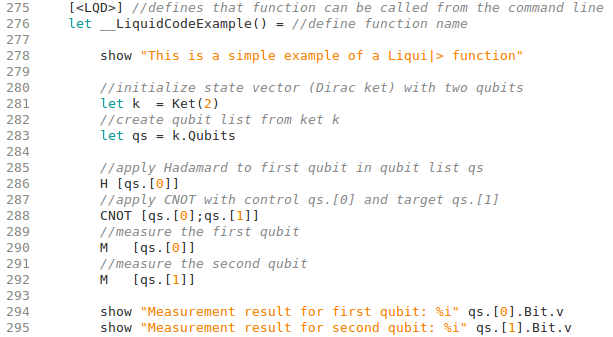
\includegraphics[scale=0.6]{img/liquidcodesnippet.png}
       \caption{\label{fig:liquidsnippet} F\# code snippet from Microsoft's quantum simulation toolsuite Liqui$\ket{}$. First, the code initialises two qubits in state $\ket{00}$ and applies an H gate to the first qubit leading to the state $\frac{\ket{00}+\ket{10}}{\sqrt{2}}$. Next, a CNOT gate, using the first and second qubit as control and target respectively, is applied. This leads to the maximally entangled state $\frac{\ket{00}+\ket{11}}{\sqrt{2}}$. Subsequently, both qubits are measured and the resulting bit values are displayed in the console.}
\end{figure}

\section{IBM Quantum Experience}
\label{subsec:ibmqc}

Since May 2016, IBM has enabled public cloud access to their experimental quantum processor containing five non-error-corrected superconducting qubits located at the IBM Quantum Lab at the Thomas J Watson Research Center in Yorktown Heights, New York \cite{ibmquantumcomputer}. Instead of only simulating on classical hardware, this opens up the possibility of executing the quantum kNN algorithm on actual quantum hardware.

The so-called IBM Quantum Experience\footnotemark[9] provides the user with access to their \emph{quantum composer} which is the main tool for algorithm design. The quantum composer shown in Fig.~\ref{fig:composer} consists of 5 horizontal lines, one for each qubit, and enables the user to choose from a universal gate set (bottom of Fig.~\ref{fig:composer}) consisting of the following 10 quantum logic gates: $\mathbb{1}$, X, Y, Z, H, S, S$^\dagger$, T, T$^\dagger$ and CNOT. Additionally, there are two different types of measurement:
\begin{enumerate}[(a)]
\item A measurement in the standard basis, resulting in a probability distribution over the \0 and \1 state.
\item A Bloch measurement that visually projects the state onto the Bloch sphere. This is achieved by performing so-called \emph{quantum state tomography}\footnotemark[10] on the qubit while ignoring possible entanglement with other qubits \cite{ibmqetomo}.
\end{enumerate}
Through simple drag and drop the user can move any of those quantum logic and measurement gates into the quantum composer to create a quantum algorithm. However, the current version of the IBM Quantum Experience only allows the application of up to 40 quantum logic and measurement gates per qubit in the composer.
\footnotetext[9]{The IBM Quantum Experience can be accessed via \url{https://quantumexperience.ng.bluemix.net/qstage/}.}
\footnotetext[10]{A detailed explanation of quantum state tomography exceeds the scope of this thesis. The interested reader is referred to \citeA{altepeter649quantum}.}

\begin{figure}[H]
      \centering
       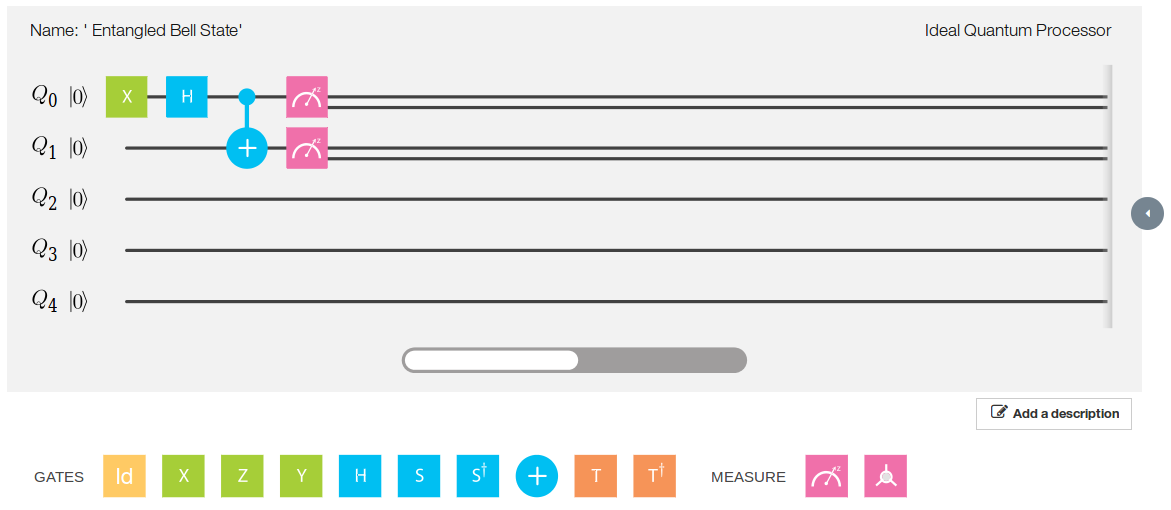
\includegraphics[scale=0.36]{img/ibmcomposer.png}
       \caption[]{\label{fig:composer} Screenshot showing the IBM Quantum Composer. For each of the five qubits $Q_0$,...,$Q_4$ there is a horizontal line with 40 available quantum gate slots. Quantum gates chosen from the universal gate set at the bottom can be dragged and dropped into the quantum composer to create a quantum algorithm.\footnotemark[11]}
\end{figure}
\footnotetext[11]{Screenshot was taken from \url{https://quantumexperience.ng.bluemix.net/qstage/#/editor}.}

After registration, each user receives a limited number of units that are required to execute algorithms on the real quantum processor. A minimum of three units is required to send the gate sequence of a composed algorithm to IBM's QC in New York. Then, depending on the waiting queue and the availability of the QC the results will be send back via email within a few minutes or days. The IBM Quantum Experience also allows for free quantum simulations under ideal or real conditions which provide a great tool for experimentation without spending user units.

The main limitation of the IBM Quantum Experience are the qubit decoherence times since they restrict the maximum number of possible operations before the qubits lose their quantum behaviour and their quantum information. Therefore, the number of quantum gates per qubit is currently limited to only 40 which essentially means 39 logic gates and one measurement gate. According to the qubit calibration results shown in Fig.~\ref{fig:calibration}, the amplitude damping times of the five qubits range from \SI{52.3}{\micro\second} to \SI{81.5}{\micro\second}. Furthermore, the phase damping times range from \SI{60.9}{\micro\second} to \SI{112.4}{\micro\second}. Currently, the implementation of a single-qubit quantum logic gate takes 130 nanoseconds (ns) and applying a CNOT gate takes 500ns \cite{ibmgatetimes}.

\begin{figure}[H]
      \centering
       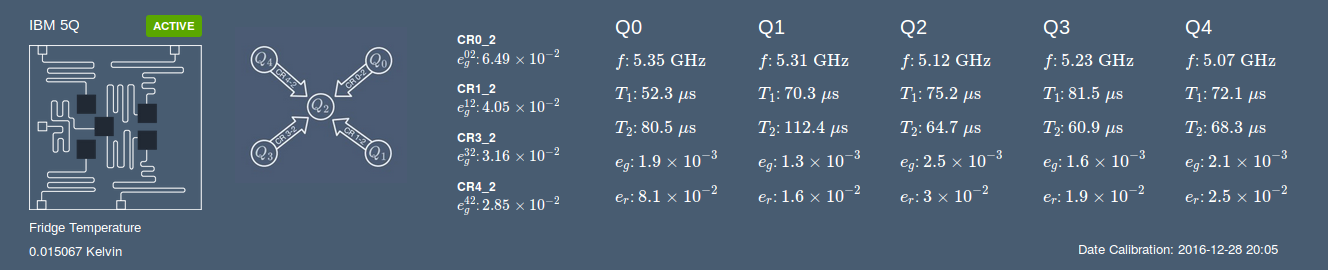
\includegraphics[scale=0.33]{img/ibmcalibration.png}
       \caption[]{\label{fig:calibration} Screenshot of IBM quantum processor calibration results showing the chip architecture, qubit arrangements, decoherence times and qubit error rates (28. December 2016 - 20:05).\footnotemark[12]}
\end{figure}
\footnotetext[12]{Screenshot was taken from \url{https://quantumexperience.ng.bluemix.net/qstage/#/editor}.}